\documentclass{article}
\usepackage[T1]{fontenc}
\usepackage[utf8]{inputenc}
\usepackage{lmodern}
\usepackage{amsmath}
\usepackage{sansmath}
\AtBeginDocument{\sansmath}
\renewcommand{\familydefault}{\sfdefault}
\usepackage[paperwidth=19cm,paperheight=14cm,margin=0.4cm]{geometry}
\usepackage{graphicx}
\usepackage{tikz}
\usetikzlibrary{positioning,fit,calc,arrows.meta,backgrounds,decorations.pathreplacing}
\pagestyle{empty}
\setlength{\parindent}{0pt}
\graphicspath{{img/}}

\definecolor{ink}{HTML}{0A0A0A}
\definecolor{muted}{HTML}{6A6A69}
\definecolor{line}{HTML}{BDBDBA}
\definecolor{red}{HTML}{E03A3A}
\definecolor{blue}{HTML}{2E6FE0}
\definecolor{yellow}{HTML}{D9A11A}
\definecolor{green}{HTML}{23A06A}
\definecolor{model}{HTML}{8C8C8A}

\tikzset{
  every picture/.style={font=\sffamily\small, line cap=round, line join=round},
  flecha/.style={-{Stealth[length=2.3mm,width=1.7mm]}, line width=0.7pt, draw=ink},
  grupo/.style={draw=#1, dash pattern=on 3pt off 2pt, line width=0.8pt, rounded corners=2pt, inner sep=6pt},
  titulo/.style={font=\sffamily\small\bfseries, text=#1, anchor=south west, inner sep=1pt},
  foto/.style={inner sep=0pt, outer sep=0pt, draw=ink, line width=0.5pt},
  caja/.style={draw=ink, line width=0.5pt, fill=#1, text=white, font=\sffamily\scriptsize\bfseries,
    text width=3.75cm, minimum height=0.46cm, align=center, inner sep=1.5pt},
  nota/.style={font=\sffamily\scriptsize, text=muted, align=center, inner sep=1pt},
  etapa/.style={font=\sffamily\footnotesize\bfseries, text=ink, align=center, inner sep=1pt},
  paso/.style={draw=ink, line width=0.5pt, fill=#1, text=ink, font=\sffamily\scriptsize, align=center,
    inner sep=3pt, minimum height=0.95cm, text width=2.35cm},
  paso/.default=white,
  grupofondo/.style={draw=#1, line width=0.8pt, fill=#1!6, rounded corners=3pt, inner sep=7pt},
  llave/.style={decorate, decoration={brace, mirror, amplitude=5pt, raise=2pt}, line width=0.7pt, draw=#1},
  llavetexto/.style={font=\sffamily\small\bfseries, text=#1, align=center},
}

\begin{document}
\begin{tikzpicture}

\node[foto] (in) at (0, -0.29) {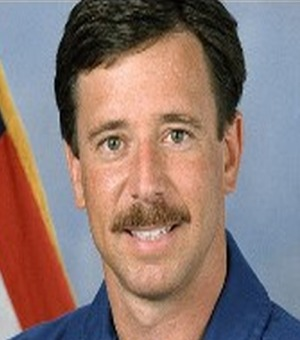
\includegraphics[width=2.05cm]{foto.jpg}};
\node[etapa, above=4pt of in] {Foto};

\node[foto] (yolo) at (2.85, 1.05) {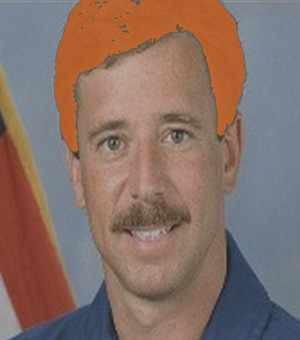
\includegraphics[width=1.45cm]{t_yolo.jpg}};
\node[nota, below=1pt of yolo] (yl) {YOLOv8 propio};
\node[foto] (mp) at (2.85, -1.3) {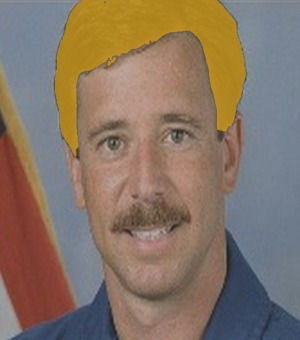
\includegraphics[width=1.45cm]{t_mediapipe.jpg}};
\node[nota, below=1pt of mp] (ml) {MediaPipe\\IoU entre ambas: 0,95};
\node[grupo=model, fit=(yolo)(yl)(mp)(ml)] (g1) {};
\node[titulo=muted] at (g1.north west) {Máscara};

\node[foto] (shade) at (6.0, 1.05) {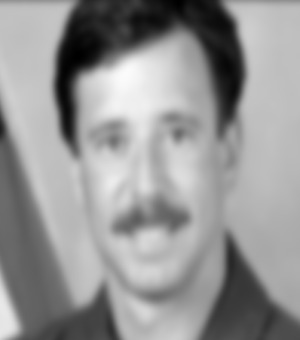
\includegraphics[width=1.45cm]{t_sombreado.jpg}};
\node[nota, below=1pt of shade] (sl) {sombreado $G_\sigma(L)$};
\node[foto] (detail) at (6.0, -1.3) {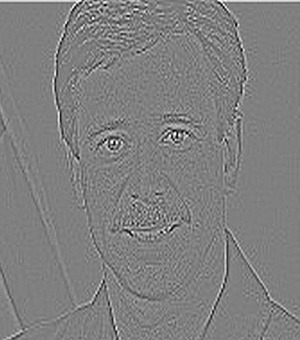
\includegraphics[width=1.45cm]{t_detalle.jpg}};
\node[nota, below=1pt of detail] (dl) {detalle $L - G_\sigma(L)$};
\node[grupo=blue, fit=(shade)(sl)(detail)(dl)] (g2) {};
\node[titulo=blue] at (g2.north west) {Luminosidad $L^*$};

\node[paso, text width=3.75cm, minimum height=2.3cm] (formula) at (9.65, -0.29) {%
  \textbf{\footnotesize Fórmula en CIELAB}\\[4pt]
  $L' = \text{base} + k\,(0{,}8\,s + 1{,}2\,d)$\\[2pt]
  $\text{base} = 0{,}72\,L_t + 0{,}28\,\bar L$\\[2pt]
  $k = \mathrm{clip}(20/s_L)$ entre 0,9 y 1,8\\[4pt]
  croma del tinte, menor en las sombras};
\node[grupo=red, fit=(formula)] (g3) {};
\node[titulo=red] at (g3.north west) {Recolorear};

\node[foto] (out) at (13.5, -0.29) {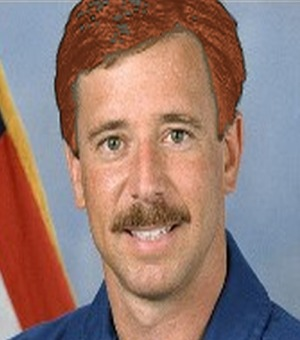
\includegraphics[width=2.05cm]{tinte.jpg}};
\node[etapa, above=4pt of out] {Resultado};

\coordinate (mid) at (0, -0.29);
\draw[flecha] (in.east |- mid) -- (g1.west |- mid);
\draw[flecha] (g1.east |- mid) -- (g2.west |- mid);
\draw[flecha] (g2.east |- mid) -- (g3.west |- mid);
\draw[flecha] (g3.east |- mid) -- (out.west |- mid);

\coordinate (base) at ($(g1.south) + (0, -0.06)$);
\draw[llave=muted] (g1.west |- base) -- (g1.east |- base)
  node[midway, below=9pt, llavetexto=muted] {Modelos};
\draw[llave=ink] (g2.west |- base) -- (g3.east |- base)
  node[midway, below=9pt, llavetexto=ink] {Implementado por el equipo};

\end{tikzpicture}
\end{document}
